\section{Simulation}
Simulations are conducted in the Gazebo simulator within the ROS environment. UAV used in experiments is the $\mu$Morus which can be found in the \textit{mmuav\_gazebo} repository \cite{gitLink}, along with its model parameters. Two experiments will be conducted with UAVs using two different methods of CoG variation.
Control parameters for the first case are chosen as follows:
\begin{equation*}
	\text{k}_x = 
	\begin{bmatrix}
		10 &  0  &  0 \\
		 0 & 10  &	0 \\ 
		 0 &  0  & 50 	
	\end{bmatrix}
	\, , \,	
	\text{k}_v =
	\begin{bmatrix}
		3.75 & 0 & 0 \\
		0 & 3.75 & 0 \\
		0 & 0 & 20
	\end{bmatrix}
\end{equation*}
\begin{equation*}
	\text{k}_R = 
	\begin{bmatrix}
		1.5 & 0 & 0 \\
		0 & 1.5 & 0 \\
		0 & 0 & 10
	\end{bmatrix}
	\, , \,
	\text{k}_\Omega = 
	\begin{bmatrix}
		0.65 & 0 & 0 \\
		0 & 0.65 & 0 \\
		0 & 0 & 1.54
	\end{bmatrix}
\end{equation*}

\noindent Rotational control parameters, in the second case, stay the same, while translational parameters are the following: 
\begin{equation*}
	\text{k}_x = 
	\begin{bmatrix}
		7.2 &  0  &  0 \\
		0 & 7.2  &	0 \\ 
		0 &  0  & 50 	
	\end{bmatrix}
	\, , \,	
	\text{k}_v =
	\begin{bmatrix}
		2.6 & 0 & 0 \\
		0 & 2.6 & 0 \\
		0 & 0 & 20
	\end{bmatrix}
\end{equation*}
For both cases, initial parameters are obtained by considering the error dynamics \eqref{error_dynamics_linear} and \eqref{error_dynamics_angular} in the equilibrium state. However, they are further tuned with better position tracking performance in mind.\\
\todo[inline]{how tuned?, lovro: for better position tracking}
It is important to note that the actuator dynamics of moving masses and manipulators is taken in consideration within the Gazebo simulation environment. Furthermore there is a slight transient delay when increasing or decreasing rotor velocity which results in a non-instantaneous control force change. \\
\indent The chosen trajectory tracking problem is formulated as a rotating spiral:
\begin{gather*}
	\textbf{x}_d(t) = [0.4\text{t}; \, 0.5\text{sin}(\pi\text{t}); \, 0.6\text{cos}(\pi\text{t}) + 2] \\
	\textbf{b}_{1,d}(t) = [\text{cos}\left(\frac{\pi}{5}\text{t}\right); \, \text{sin}\left(\frac{\pi}{5}\text{t}\right); \, 0]
\end{gather*}
\noindent In both experiments trajectory lasts for 20s. Initial position and orientation is chosen at the start of the trajectory. \\

\begin{figure}[h!]
	\centering
	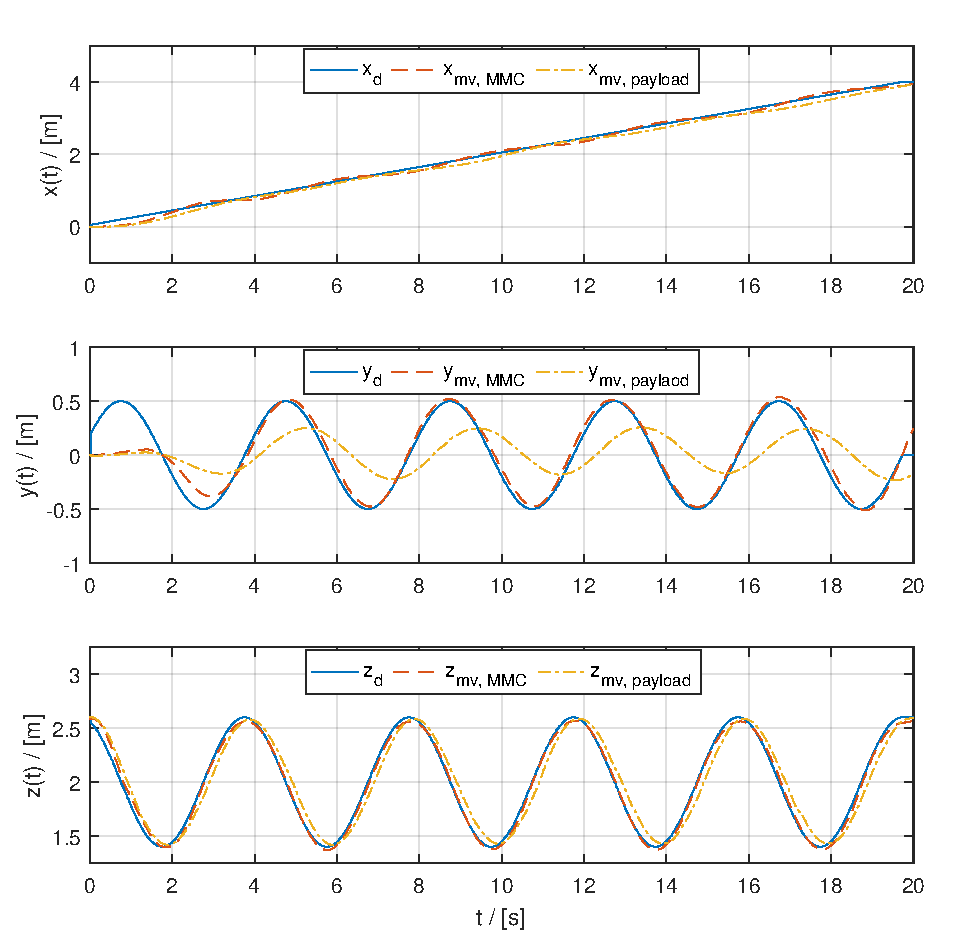
\includegraphics[width=\columnwidth]{./pictures/both_pos.pdf}
	\caption{\todo[inline]{Add text...}}
	\label{fig:traj_pos}
\end{figure}

\begin{figure}
	\centering
	\begin{minipage}{0.5\columnwidth}
		\centering
		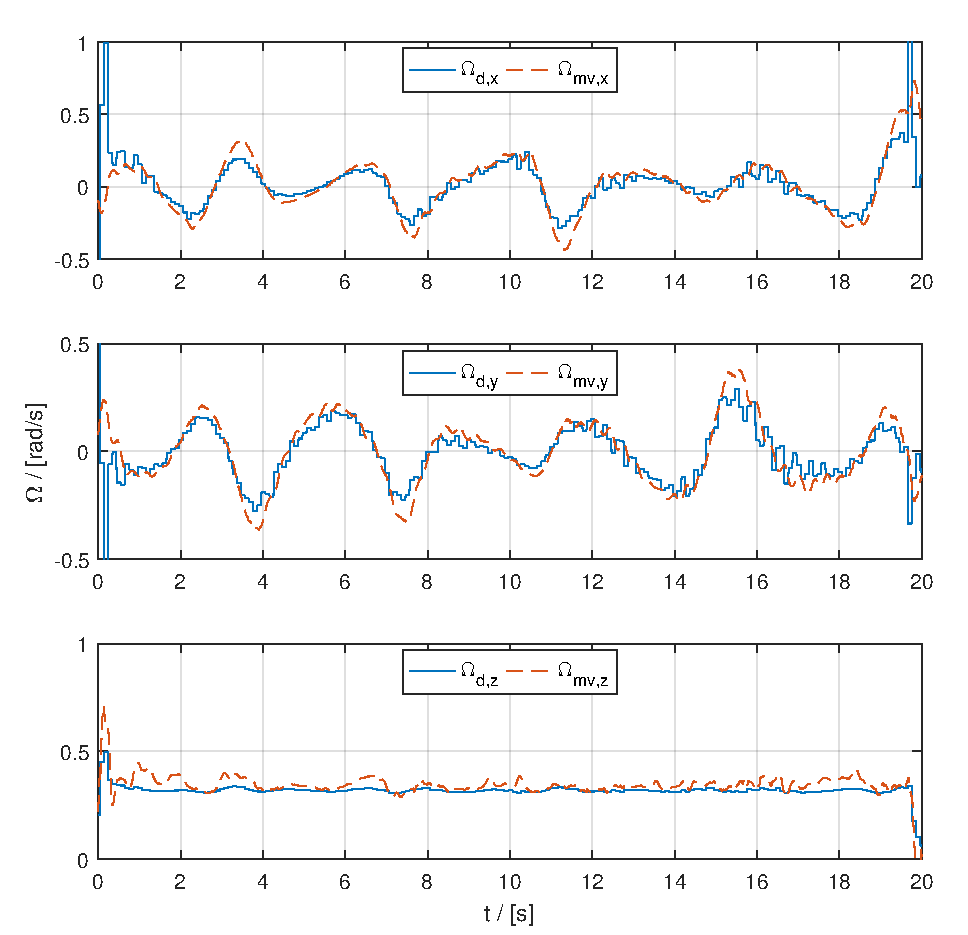
\includegraphics[width=\columnwidth]{./pictures/mmcuav_omega.pdf}
		\caption*{a)}
		\label{fig:mmcuav_omega}
	\end{minipage}%
	\begin{minipage}{0.5\columnwidth}
		\centering
		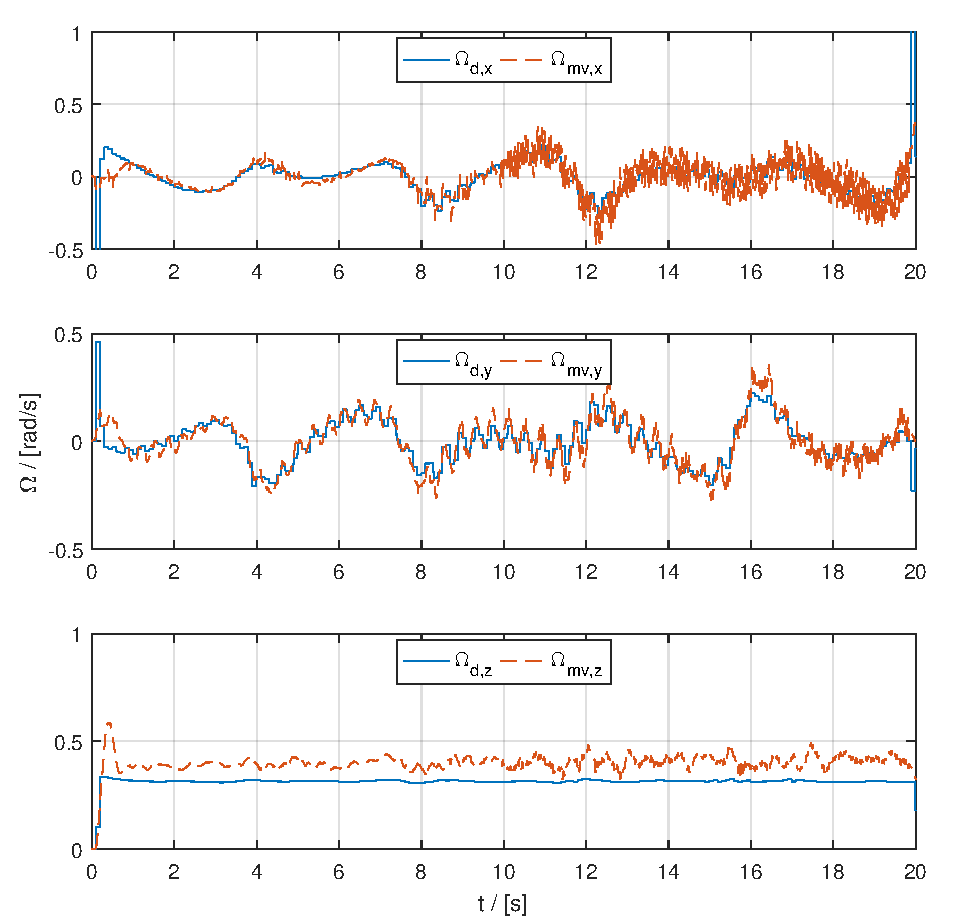
\includegraphics[width=\columnwidth]{./pictures/mmuav_omega.pdf}
		\caption*{b)}
		\label{fig:mmuav_omega}
	\end{minipage}
	\caption{\todo[inline]{Add text...}}
\end{figure}

\begin{figure}
	\centering
	\begin{minipage}{0.5\columnwidth}
		\centering
		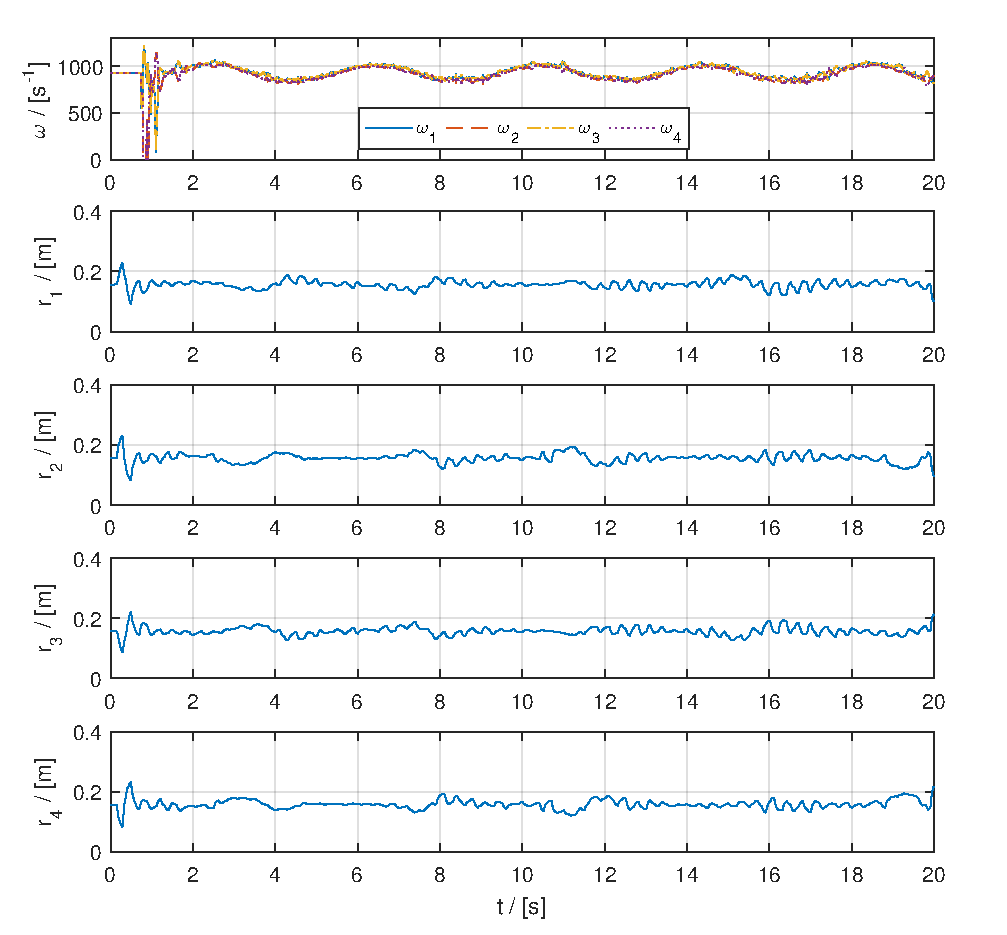
\includegraphics[width=\columnwidth]{./pictures/mmcuav_control_inputs.pdf}
		\caption*{a)}
		\label{fig:mmcuav_control}
	\end{minipage}%
	\begin{minipage}{0.5\columnwidth}
		\centering
		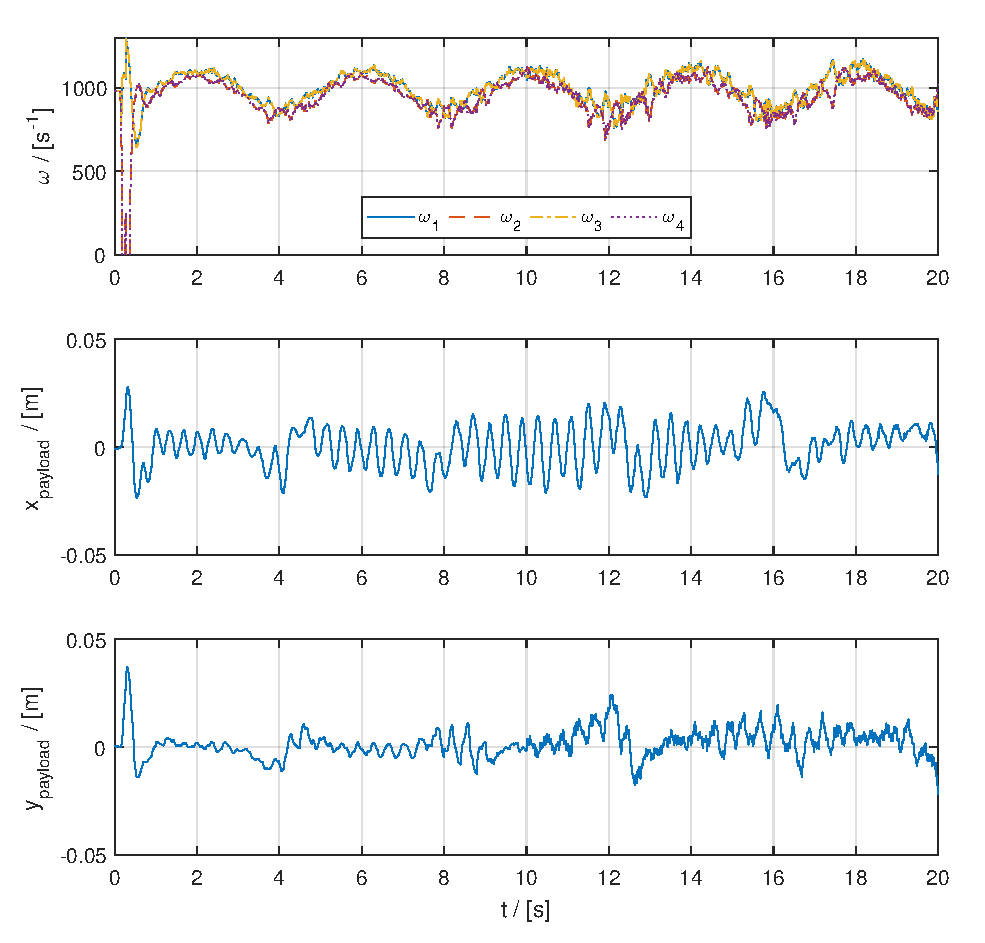
\includegraphics[width=\columnwidth]{./pictures/mmuav_control_inputs.pdf}
		\caption*{b)}
		\label{fig:mmuav_control}
	\end{minipage}
	\caption{\todo[inline]{Add text...	}}
\end{figure}


\begin{figure}[h!]
	\centering
	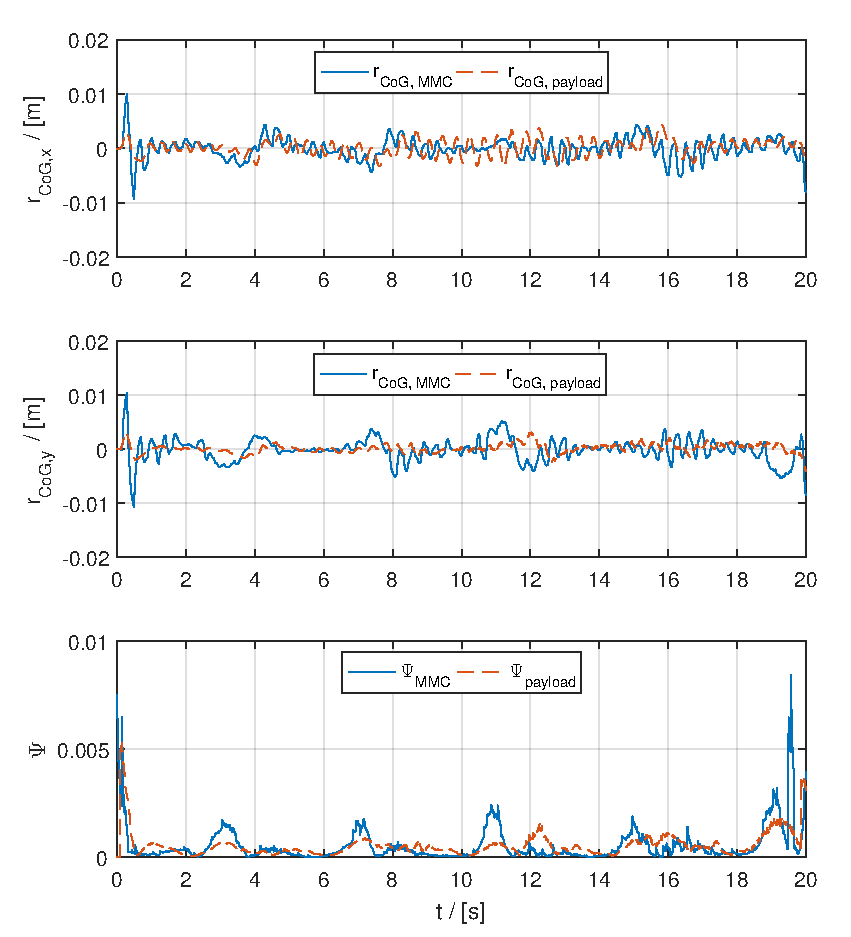
\includegraphics[width=\columnwidth]{./pictures/both_cog_err.pdf}
	\caption{\todo[inline]{Add text...}}
	\label{fig:cog_error}
\end{figure}

\todo[inline]{TODO: komentirati sve rezultate.}
\todo[inline]{TODO: dodati MSE za trajektorije}